% Bascically just an adaption of Todd Davies flashcards for the subjects,
% with plans to basically expand upon them

\documentclass[frontgrid,a4paper]{flacards}
\usepackage{color}
% For funky database symbols
\usepackage{newlfont}
\usepackage{tabularx}
\usepackage{graphicx}


\definecolor{light-gray}{gray}{0.75}
\fboxsep=20pt

\newcommand{\frontcard}[1]{\fboxsep=2pt\textcolor{light-gray}{\colorbox{light-gray}{$#1$}}}
\newcommand{\backcard}[1]{#1}
\newcommand\tab[1][0.5cm]{\hspace*{#1}}

\newcommand{\flashcard}[1]{% create new command for cards with blanks
    \card{% call the original \card command with twice the same argument (#1)
        \let\blank\frontcard% but let \blank behave like \frontcard the first time
        #1
    }{%
        \let\blank\backcard% and like \backcard the second time
        #1
    }%
}

\begin{document}

\pagesetup{2}{4} 

\card{
	What is $\sigma$?
}{
	The selection operator (selects rows).
}

\card{
	What is $\pi$?
}{
	The projection operator (selects columns).
} 

\card{
	What is $\delta$?
}{
	The distinct operator (makes sure no rows are repeated).
}

\card{
	What is $\times$?
}{
	The product operator (produces all permutations of the rows of two tables).
}

\card{
	What is $\Join$?
}{
	The join operator (natural or otherwise, it joins two tables together based
	on a column).
}

\card{
	What is $\rho$?
}{
	The rename operator (renames column names).
}

\card{
	What are the three layers of DBMS abstraction?
}{
	Physical, logical and view
}

\card{
	Name three DBMS interface languages
}{
	\begin{tabularx}{0.32\textwidth}{l X}
		- & DDL: Data Definition Language\\
		- & DML: Data Manipulation Language\\
		- & DQL: Data Query Language\\
	\end{tabularx}
}

\flashcard{
	To select the age column from the people table without duplicates you would do:\\
	\texttt{SELECT \blank{DISTINCT} \blank{age} FROM \blank{people};}
}

\flashcard{
	To select all the columns of people who are above 50 you would do:\\
	\texttt{SELECT * FROM \blank{people} WHERE \blank{age > 50};}
}

\flashcard{
	To select all the columns of people who are between 20 and 40 you would do:\\
	\texttt{SELECT * FROM \blank{people} WHERE \blank{age BETWEEN 20 AND 40};}
}

\card{
	What are the three SQL set operations?
}{
	UNION, EXCEPT \& INTERSECT
}

\card{
	What is the SQL syntax to join 2 tables on a certain column name?
}{
	\texttt{
		SELECT * \\
		FROM table1 JOIN table2 \\
		USING (<column-name>);
	}
}

\card{
	What is the SQL syntax for a natural join on 2 tables?
}{
	\texttt{
		SELECT *\\
		FROM table1 NATURAL JOIN table2;
	}
}

\card{
	What is the SQL syntax for renaming tables? 
}{
	\texttt{
		SELECT *\\
		FROM table1 as a, table2 as b\\
		WHERE a.col > b.col;
	}
}

\card{
	What is the SQL syntax for sorting rows by a column value
}{
	\texttt{
		SELECT *\\
		FROM table1\\
		GROUP BY <column-name>;
	}
}

\flashcard{
	To select the average salary from the workers table you do:\\
	\texttt{SELECT AVG(salary) FROM workers}
}

\flashcard{
	To select the number of distinct salaries from the workers table you do:\\
	\texttt{SELECT COUNT(DISTINCT salary) FROM workers}
}

% NEED TO ADD MORE SQL FLASHCARDS HERE

\card{
	What are the three main constructs in ER modelling?
}{
	Entity types, attribute types \& relationship types.
}

\card{
	What type of attribute is the following?\\
	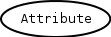
\includegraphics{images/simpleAttribute.png}
}{
	Simple attribute
}

\card{
	What type of attribute is the following?\\
	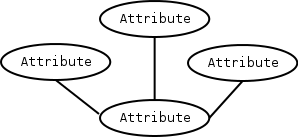
\includegraphics[scale=0.6]{images/compositeAttribute.png}
}{
	Composite attribute
}

\card{
	What type of attribute is the following?\\
	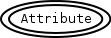
\includegraphics{images/multiAttribute.png}
}{
	Multi-valued attribute
}

\card{
	What type of attribute is the following?\\
	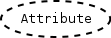
\includegraphics{images/derivedAttribute.png}
}{
	Derived attribute
}

\card{
	What type of entity is the following?\\
	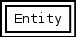
\includegraphics{images/weakEntity.png}
}{
	Weak entity
}

% RELATIONSHIP FLASHCARDS NEED ADDING

\card{
	Explain normalization
}{
	The process of decomposing unsatisfactory relations by creating smaller relations from them.
}

\card{
	What does the normal form indicate?
}{
	The quality level of the database schema
}

\card{
	What does 1NF mean?
}{
	This is a relation in its first normal form, where every field contains only atomic values.
}

\flashcard{
	The main technique we use to try and refine schema is \blank{decomposition}.
}

\card{
	What allows us to access one row of an SQL command at a time and iterate over the rows?
}{
	A cursor
}

\flashcard{
	Triggers are constructs that react to certain conditions. They obey an \blank{event-condition-action} model.
}

% MORE TRIGGER STUFF HERE!!!!!!

\card{
	What is a transaction?
}{
	An action or series of actions carried out by the user that read or update the contents of the database.
}

\card{
	What happens if a transaction fails?
}{
	The database is rolled back to it's most recent consistent state.
}

\card{
	What are a transactions four basic properties?
}{
	\begin{tabularx}{0.32\textwidth}{l X}
		1. & Atomicity\\
		2. & Consistency\\
		3. & Isolation\\
		4. & Durability\\
	\end{tabularx}
}

\card{
	In terms of transaction, what does atomicity mean?
}{
	A transaction must either complete all work or else it must be as if no partial work was ever done.
}

\card{
	In terms of transaction, what does consistency mean?
}{
	A transaction must transform databases from one consistent state to another.
}

\card{
	In terms of transaction, what does isolation mean?
}{
	Partial effects of incomplete transactions should not be visible to other transactions.
}

\card{
	In terms of transaction, what does durability mean?
}{
	The effects of a committed transaction are permanent and must not be lost because of later failure.
}

\card{
	What is concurrency control?
}{
	The process of managing simultaneous operations on the database without allowing them to interfere with one another.
}

\card{
	When does a `lost update problem' occur? How do you solve it?
}{
	When a user's update overwrites another user's update. Mitigated by stopping concurrent operations from reading objects/tables while another operation is writing to it.
}

\card{
	When does an uncommitted dependency problem occur? How do you solve it?
}{
	When one transaction can see the immediate results of another transaction before it has committed. Mitigate this by stopping reads from occurring on objects that haven't been committed.
}

\card{
	When does an inconsistent analysis problem occur? How do you solve it?
}{
	When a transaction $A$ reads values that transaction $B$ has updated during transaction $A$ occurs. Mitigate this by stopping one transaction from reading while another is updating and vice versa
}

\card{
	What does serializability guarantee?
}{
	Sequences of execution that will ensure consistency
}

\card{
	What is a schedule?
}{
	A set of reads and writes to the database by concurrent transactions.
}

\card{
	What is a serial schedule?
}{
	This is when reads and writes must be executed consecutively with no interleaving operations.
}

\card{
	What is a non-serial schedule?
}{
	One where any operations can be interleaved?
}

\flashcard{
	To make the database as efficient as possible we want to find as many \blank{non-serial} schedules as we can so that we can get \blank{parallel} computation.
}

\flashcard{
	The two most basic control techniques are \blank{locking} and \blank{timestamping}.
}

\card{
	What is locking?
}{
	This is when data items are locked to prevent other transactions from viewing or updating them.
}

\flashcard{
	Transactions must obtain a \blank{shared} lock on a data item when it wants to read.
}

\flashcard{
	Transactions must obtain an \blank{exclusive} lock when it wants to write.
}

\flashcard{
	Locks are assigned using the \blank{two-phase-locking} protocol.
}

\flashcard{
	The two phases in the two-phase-locking protocol are the \blank{growing} phase and the \blank{shrinking} phase.
}

\card{
	What happens in the growing phase of the two-phase-locking protocol?
}{
	The transaction my acquire locks but cannot release them.
}

\card{
	What happens in the shrinking phase of the two-phase-locking protocol?
}{
	The transaction my release locks but cannot acquire them.
}

\card{
	How can cascading rollback be prevented?
}{
	By ensuring that locks are only released at the end of transactions.
}

\card{
	What should happen if deadlock occurs?
}{
	One or more of the transactions should be aborted and restarted.
}



\end{document} 
